\documentclass[a4paper,usenames,dvipsnames,table]{report}
\usepackage[utf8]{inputenc}
\usepackage{amsmath}
\usepackage{amsfonts}
\usepackage{amssymb}
\usepackage{multirow}
\usepackage{graphicx}
\usepackage{fancyhdr}
\usepackage{hyperref}
\usepackage{float}
\usepackage{color}
\usepackage{booktabs}
\usepackage[usenames, dvipsnames]{xcolor}
\usepackage[top=2cm, margin=2.5cm]{geometry}
\usepackage{titlepic}
\usepackage{mathtools}

% \usepackage{eurosym}

\graphicspath{{images/}}
\newcommand{\warning}[2] {
    \textcolor{red}{(#1) #2}
}
\let \smalland \land
\let \smallor \lor
\newcommand{\bigand}[1] {\bigwedge_{#1}}
\newcommand{\bigor}[1] {\bigvee_{#1}}



\begin{document}

% title configuration
\title{
    {\Huge \textbf{Lab assignment \#2: Logical Satisfiability and Heuristic Search\\}}
    {\Large Heuristics \& Optimization 2017-2018 (Group 89)}
}
\author{
    Álvaro Cáceres Muñoz ({\normalsize \href{mailto:100303602@alumnos.uc3m.es}{100303602@alumnos.uc3m.es}})\\
    Guillermo Escobero Hernández ({\normalsize \href{mailto:100346060@alumnos.uc3m.es}{100346060@alumnos.uc3m.es}})\\
}
\date{}
\titlepic{
\includegraphics[width=0.5\textwidth]{uc3m.png}}




\maketitle
\tableofcontents
\chapter{Introduction}
\label{chapter: introduction}

% brief introduction explaining document contents
\section{About this lab assignment}

\paragraph{}
This document contains the report of the work carried out in this lab assignment. It is related with Logical Satisfiability and Heuristic Search. There are two main parts for this lab assignment, that are organized as follows:

\begin{itemize}
	\item Part 1 deals with the modelling of a parking problem, similar to the famous board game Rush Hour, by solving it as a SAT problem. This part has been implemented using Java and JACoP,  a library for constraint programming.
    
	\item Part 2 deals with determining the necessary sequence of movements to reconfigure the parking into a different configuration given. This is solved using the heuristic search algorithm A*.
    
\end{itemize}

\section{Document contents}

\paragraph{}
This document has been divided in four chapters, following the format requested by our professor. The following list explains what does each chapter show:

\begin{itemize}
	\item Chapter \ref{chapter: introduction} (this one) explains the contents of the document. It serves as a reference for rapid lookup across this report.
    
	\item In chapter \ref{chapter: models description}, the models of the two proposed problems are discussed.
    
	\item Chapter \ref{chapter: analysis of results} analyzes the solutions yielded both for Part 1 and Part 2 problems. 

	\item Chapter \ref{chapter: conclusions} explains the difficulties we have faced while completing this lab assignment, both from a technical and a conceptual standpoint. It also describes what have we learned (or remembered) thanks to this lab assignment.
	
\end{itemize}
\chapter{Models Description}
\label{chapter: models description}








%----------------------------------------- PART 1 --------------------------------------------------

\section{Part 1: SAT verification of the parking configuration}

\paragraph{}
For this part we had to refrain ourselves from the temptation of modelling the
problem as an assignment of cars to park positions, since these positions were
already fixed. Instead, we have to somehow \textit{check} that an (already
present) assignment was correct. In other words, the configuration read from the
input file should not be changed; JaCoP should not decide which values to assign
to the boolean variables that describe the parking. We have to make these values
\textit{fixed}, expressing this with propositional logic. One way we thought to
solve this problem is to include this information as disjunctions of only one
literal, and adding each one them to the CNF with a conjunction.


\subsection{Variables}

\paragraph{}
Variables have been defined as follows:
\begin{itemize}
  \item $c_{ij}$: there is a car at lane $i$ and position $j$
  \item $b^{d)}_{ij}$: car adjacent to that at $i,j$ entered the lane before
  \item $s^{d)}_{ij}$: car adjacent to that at $i,j$ has a category with the same waiting time
  \item $l^{d)}_{ij}$: car adjacent to that at $i,j$ has a category with lower waiting time
\end{itemize}
Where $d \in {L,R}$. $L$ represents information about the adjacent car at the left of car at $i,j$, and $R$ represents information about the adjacent car at the right of car at $i,j$.

\subsection{Propositional formula}

\paragraph{}
The formula can be divided in two parts: the part that checks for blocked cars, and the part that represents the parking configuration by using 1-variable clauses. It should be noticed that literals in the formula may be non-negated ($b^L_{ij}$) or negated ($\neg b^d_{ij}$), depending on the input file configuration. Since it would be incorrect to include a single formula (as literals on the right are non-negated or negated depending on the input file), the following equation represents a group of formulas, hence the use of set notation for the right part.

\paragraph{}
Therefore we get the following propositional formula:
\begin{equation}
  \bigand{\substack{i \in N,\\ j \in (0, N-1)}}l^{L)}_{ij} \lor (s^{L)}_{ij} \land b^{L)}_{ij}) \lor l^{R)}_{ij} \lor l^{R)}_{ij} \lor (s^{R)}_{ij} \lor b^{R)}_{ij})
  \bigand{\substack{
      \alpha \in\\
      B^{L)} \cup
      B^{R)} \cup \\
      S^{L)} \cup
      S^{R)} \cup \\
      L^{L)} \cup
      L^{R)} \cup \\
      C
    }}
    \alpha
\end{equation}
where
\begin{itemize}
  \item $B^{L)}$: matrix containing literals $b^{L)}_{ij}$ or $\neg b^{L)}_{ij}$ as loaded from the input file
  \item $S^{L)}$: matrix containing literals $s^{L)}_{ij}$ or $\neg s^{L)}_{ij}$ as loaded from the input file
  \item $S^{R)}$: matrix containing literals $s^{R)}_{ij}$ or $\neg s^{R)}_{ij}$ as loaded from the input file
  \item $L^{L)}$: matrix containing literals $l^{L)}_{ij}$ or $\neg l^{L)}_{ij}$ as loaded from the input file
  \item $L^{R)}$: matrix containing literals $l^{R)}_{ij}$ or $\neg l^{R)}_{ij}$ as loaded from the input file
  \item $C$: matrix containing literals $c_{ij}$ or $\neg c_{ij}$ as loaded from the input file
\end{itemize}

\paragraph{}
Turning this formula into CNF we get the following:
\begin{equation}
  \bigand{\substack{i \in N,\\ j \in (0, N-1)}}
  (l^{L)}_{ij} \lor l^{R)}_{ij} \lor s^{L)}_{ij} \lor s^{R)}_{ij}) \land
  (l^{L)}_{ij} \lor l^{R)}_{ij} \lor s^{L)}_{ij} \lor b^{R)}_{ij}) \land
  (l^{L)}_{ij} \lor l^{R)}_{ij} \lor s^{R)}_{ij} \lor b^{L)}_{ij}) \land
  (l^{L)}_{ij} \lor l^{R)}_{ij} \lor b^{L)}_{ij} \lor b^{R)}_{ij})
  \bigand{\substack{
      \alpha \in\\
      B^{L)} \cup
      B^{R)} \cup \\
      S^{L)} \cup
      S^{R)} \cup \\
      L^{L)} \cup
      L^{R)} \cup \\
      C
    }}
    \alpha
\end{equation}

\paragraph{}
Notice that the formula does not check literals related to the sides of the parking lot, since these are never going to be blocked.

%----------------------------------------- PART 2 --------------------------------------------------

\section{Part 2: Heuristic Search}

\paragraph{}
In this problem we are asked to move cars in a parking with an initial
configuration to get to a final configuration given. Cars can only perform
specific moves.

For solving this problem, we have used a Python3 implementation of the well-known
A* algorithm. This is an algorithm of heuristic search. In the following
sections the model and parameters used are explained.

\subsection{States}

\paragraph{}
We have decided to use parking configurations as states for the A* heuristic
search algorithm.
Each state of the problem is a different configuration of the cars in the parking
provided.

States are implemented as a class 'State', which includes a parking
configuration, a reference to its parent node, H value and G value.


\subsection{Operators}

\paragraph{}
When expanding a node, we calculate all the possible movements of the cars in
the parking. For each possible movement of each car, one node is generated. This
node contains the map after each movement. This is done by 'children' function,
that returns the child nodes after expanding a given node.

We want to point that only one movement of one car is allowed in a state change.

Also, each movement has associated a cost for performing it following the
statement requirements. When a operator is used, the cost (G) is saved.

\subsection{Initial state}

\paragraph{}
The initial state corresponds to the initial configuration of the parking
(a.k.a. first input file).
We save the data of this file in a matrix of Car objects.

\subsection{Final state}

\paragraph{}
The final state corresponds to the final configuration of the parking
(a.k.a. second input file).


\subsection{Heuristic function}

\paragraph{}
We have used Manhattan distance as the heuristic function. The distance is based
on a strictly horizontal and/or vertical path. This is based on the sum of each
distance of the current position of each car to its final position (H value).

\chapter{Analysis of results}
\label{chapter: analysis of results}








%----------------------------------------- PART 1 --------------------------------------------------

\section{Part 1: SAT verification of the parking configuration}

\subsection{Resolution and analysis of test cases}

\paragraph{}
Here it is a simple description of what each test case attempts to prove:
\begin{itemize}
  \item Case 1 proves the program finds unsatisfiable parking configuration; only one blocked car should suffice to make the configuration unsatisfiable. Car A1 is clearly blocked, so the problem is unsatisfiable. The program reports this as expected.
  \item Case 2 shows a satisfiable parking configuration. No cars are blocked in this case. The program reports this as expected.
  \item The rest of test cases show how the problem \textit{scales} in terms of execution time.
\end{itemize}

\paragraph{}
For tests 3 and above, we have used configurations with increasing number of parking positions, calculated as $M \times N$ (10, 50, 100, 500, 1000, 5000, 10000, 50000, 100000, and 500000). In order to let our computer experiment with more complex problems that require more memory, we have added some extra parameters to \texttt{java} for the \texttt{run.sh} script as follows: \texttt{-XX:-UseGCOverheadLimit -Xmx8000m}.

\paragraph{}
We used a personal computer for getting the execution times. Its technical specifications can be seen on table \ref{tab:computer specs}.
\begin{table}[H]
    \centering
    \rowcolors{2}{gray!25}{white}
    \setlength{\arrayrulewidth}{.1em}
    \setlength\extrarowheight{0.6em}
    \begin{tabular}{M{0.15} M{0.15} M{0.15} M{0.15} M{0.15}}
        \rowcolor{gray!60}
        \hline
        Model & CPU & RAM & Disk & OS\\
        \hline
        Lenovo X270 &
        Intel Core i5-7200U @ 2.50GHz &
        16 GB DDR4 &
        Crucial M300 SSD, 525 GB &
        Ubuntu Studio 16.04 LTS w/ real time kernel\\
        \hline
    \end{tabular}
    \caption{Part 1 benchmark: computer technical specifications}
    \label{tab:computer specs}
\end{table}

\paragraph{}
Figure \ref{fig:part 1 benchmark} shows how the execution time grows with respect to the dimensions of the parking lot.
\begin{figure}[H]
    \caption{Part 1 benchmark: time evolution across different input files}
    \centering
    \label{fig:part 1 benchmark}
    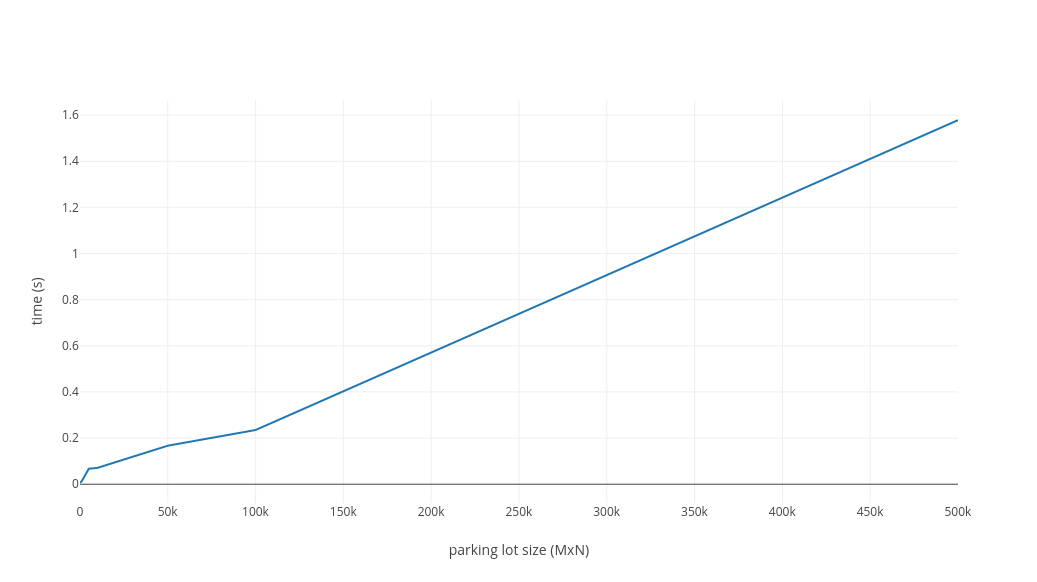
\includegraphics[width=0.7\textwidth]{images/partOneBenchmark}
\end{figure}
This time only measures calls to \texttt{DepthFirstSearch} and \texttt{SimpleSelect} functions from the \texttt{JaCoP} library; that is, it doesn't include the initialization of the boolean variables and literals. We could not finish trying with an input size of 1000000, but it lasted for a considerably larger amount of time compared to previous input sizes before running out of heap space (which had already been expanded with the java arguments we commented before). This difference in execution time with respect to former input sizes makes us think that this problem may follow a close-to-exponential time complexity; that would make sense, since JaCoP uses DFS to look for a satisfiable set of assignments. DFS takes a linear amount of memory, but it uses an exponential amount of time.

%----------------------------------------- PART 2 --------------------------------------------------

\section{Part 2: Heuristic Search}

\subsection{Resolution and analysis of test cases}

\paragraph{}
As will be explained in the conclusions, we have encountered some problems
implementing A*.

In this part some tests are performed and discussed. We are including very
simple scenarios in this report, because, as will be explained in the
conclusions, we have encountered some problems implementing A*.

Our implementation solves problems that can found the goal expanding the first
node (initial state).

\chapter{Conclusions}
\label{chapter: conclusions}

\section{On the difficulty of this lab assignment}

\paragraph{}
We were surprised about the time we had to spend in Part 1, especially knowing this part is arguably the easiest of the two requested for this lab assignment. Firstly, we had a tough time thinking how to model the problem as a SAT problem; we were blinded by the idea of assigning car positions in the parking, while the problem was to simply check if the (already assigned) cars were not blocked. Secondly, we spent more time than we would have wanted because of implementation details; at some point we experimented the need to perform a good refactoring to our code.

\paragraph{}
With Part 2, the implementation was pretty straightforward, and Python's simple syntax was of great help for us to have our program up and running in no time. However, no matter how well did the program work, we know that the difficulty of this second part relies on how do we design states, operators and the heuristic function. In this way, and once we had our implementation ready, we spent most part of our time (considerably more than implementing the program) simply changing the heuristic function and related details.

\section{On the knowledge we have acquired and/or reinforced}

\paragraph{}
This lab assignment has made us look at SAT from a different point of view. We have found Part 2 of the lab assignment quite useful, since modelling the requested problem as a search problem is a skill we still have to acquire by practice. This lab assignment has served as a perfect search exercise with regard to the final exam we have in January, where we will have for sure an exercise on search.

% back cover
\newpage\null\thispagestyle{empty}\newpage

\end{document}
